\chapter{Introduction}
\label{chap:intro}

The introduction to your document should lead your
readers into your report and give them an idea of what to expect.
You should
begin with a general statement about the topic before moving on
to specific issues. This strategy will help make the content
accessible to your readers, especially those who are not specialists
in the field. Illustrations, like Figure~\ref{fig:halwin}, often
help to introduce the reader to the problem (from  \parencite{kjeldsen05cor}).

\floatingfigure{Graphics/halden-window}{0.6}{Example of a window query in a map (map from www.finn.no)}
\label{fig:halwin}


In the introduction, you should do the following, in approximately this order:
\begin{compactitem}
  \item State the subject of your document as clearly as possible, and briefly explain why you are doing it (motivation)
    \item Provide necessary and relevant background information (you will elaborate on this matter in Chapter \ref{chap:analysis}, Analysis)
  \item Define the problem you are addressing, your approach to the problem, and why this problem is important
  \item Define the scope of your work (in particular limitations and things you will {\em not} deal with)
  \item Describe your research method, i.e., how you are going to proceed to answer your research question
  \item Give an outline of the rest of the document
\end{compactitem}

You should think of the introduction  as the foundation of your master work, and accordingly you should put considerable efforts in getting it right. 


\section{Background and motivation}
\label{sec:background-motivation}

Here you will describe the topic of your research in broad terms, so that even your grandfather should be able to get the general picture. If you are cooperating with a company, research institute, etc., they should also be introduced. It is also important that you explain {\em why} your topic is interesting and worth researching.

\lipsum[11-14]


\subsection{Research question/Problem statement/Objectives}
\label{sec:research-question}

Every academic paper needs a clearly stated goal, concisely describing its purpose. The formulation depends on the type of document. Here we will see how it can be done in a bachelor’s and master’s thesis. You should put considerable effort in describing your goals, since they will be governing the rest of your work. However, goals may change during the projects, and may need revision now and then.

\paragraph{Bachelor}

A bachelor project is generally more practically oriented than a master’s thesis. Often, the pro-ject has an external project owner, like a company or an institution. The goal will be to provide something that can gain the project owner in some way. Hence, it is important to formulate the effects project owner want to achieve. Objectives often starts with “To\dots”.
The following is from a project developing a social trading app for exchanging used books  \parencite{akeriversen20bah}:

\begin{description}
\item [Objective 1] To connect people that enjoy books with each other.
    \begin{description}
    \item [Objective 1.1] To connect people that enjoy books with each other.
    \item [Objective 1.2] To lessen the environmental effect that printing a new book has.
    \end{description}
\end{description}

If the bachelor project is more theoretically oriented, the goals could be stated as in a master’s thesis, as described in the following section.

\paragraph{Master}

A research question\footnote{It is common with more than one question} is a formal statement of the goal of a study. The research question should clearly and concisely state what the study will investigate or attempt to prove. 
Good research questions help to focus the research and the writing by providing a red thread through the project and the report. 

The research question will surface both in the analysis of the problem, the choice of methods, the design and implementation of the project, and,  most importantly, it will be revisited in the discussion and conclusion parts of the report.

The following example is from  \parencite{killerud14sgs}:

\begin{quotation}
As mentioned, opportunities arise with smart-phones for providing feedback on electricity consumption when coupled with a smart meter. A display such as the eWave, shown in Figure \ref{fig:display}, requires that a user take it upon themselves to check their consumption regularly. An application that notifies the user when consumption is high on a device that, for most parts of the day, is within reach of its owner does not require this initiation. However, it is not certain how such notifications will affect or be perceived by users. Further on in the report I attempt to shed some light on this.
My research question consists of two parts. First, I wish to shed some light on the user experience:


\begin{description}
\item [RQ 1] Given immediate feedback on changes in the electricity consumption through their mobile phone, how do users respond?
\end{description}

Secondly, I wish to see if there is a trend towards a lowering of the electricity consumption peak:

\begin{description}
\item [RQ 2]  What impact does a mobile phone assistant have on electricity consumption patterns in an effect-based billing situation?
\begin{description}
\item [RQ 2.1] You may elaborate in a secondary research question.
\end{description}
\end{description}

\begin{figure}[!htbp]
    \center
    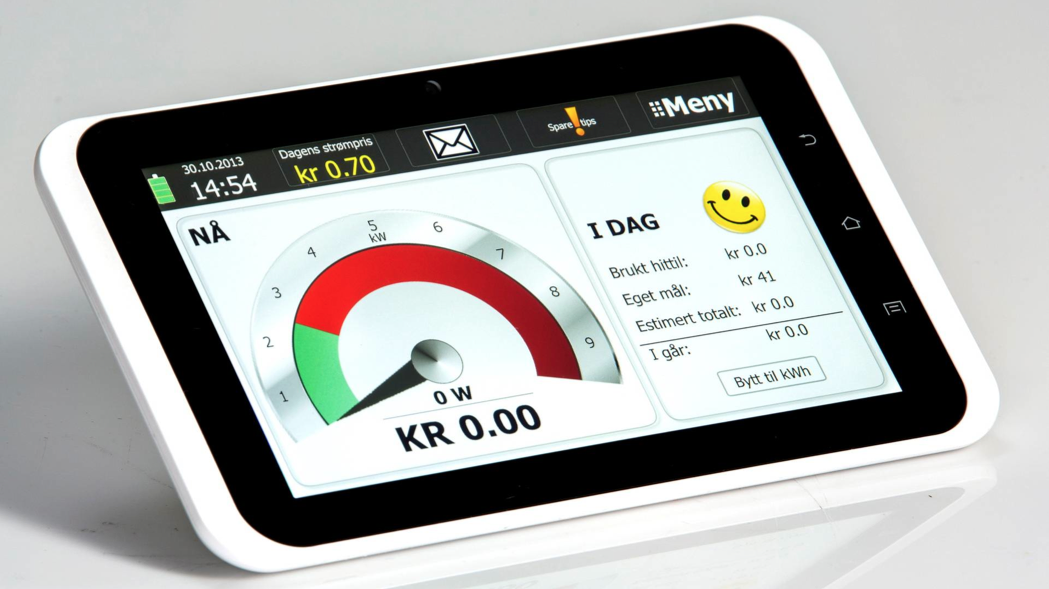
\includegraphics[width=0.6\textwidth]{Graphics/display}
    \caption{The eWave display being offered to Fredrikstad Energi’s customers. The display is 7 inches across, and is based on the Android platform (photo by Odin Media).}
    \label{fig:display}
\end{figure}

\end{quotation}

\subsection{Method}
\label{sec:method}

Here you shall explain how you are going to find answers to the research questions. 
The research method should be treated in more detail later in the report.
Here is an example from  \parencite{nordenhaug11hmf} (it is somewhat sketchy, it is OK to be more detailed than this):

\begin{quotation}
The concept described in this thesis has evolved throughout the work with it, taking on an explorative approach. This process has been incremental using several rounds of iteration before ending
up as a working prototype tested in a real-life setting, involving potential end users throughout the design.
The below mentioned methods have been used in the process:

\begin{compactitem}
\item Identification of research objectives
\item Literature and case studies
\item Development of mock-up videos
\item Implementation of a high-fidelity prototype
\item Field test and interview
\item Testing the prototype on real representative users
\end{compactitem}
\end{quotation}

\subsection{Deliverables}
\label{sec:deliverables}

Here you describe the tangible outcomes of your projects. This obviously includes the thesis, in addition to software, prototypes and such.

\lipsum[7-9]

\section{Report Outline}
\label{sec:outline}

The last point in the introduction is an outline of the rest of the report, for example like this (from  \parencite{kjeldsen05cor}):

\begin{quotation}
Chapter 2 provides background information on range search and line simplification. In the section concerning range search, several data structures and algorithms are presented. The second section describes some of the different techniques developed for performing completely automated line simplification procedures. Finally, another proposed approach to combining the two problems is presented.

The third chapter gives a general description of the PST and what it can be used for. The interval
stabbing problem is an important aspect of the work presented in this thesis, and the third chapter
explains how to solve this with a PST. Next, the interval stabbing problem is expanded to a ``grid
stabbing problem”, which also can be solved using a PST, and the reason for this is described. Chapter 4 gives a detailed description of the new data structure and the search methods that
have been developed. After this, theoretical analyses are provided. This chapter also explains how
an external version of it has been implemented, along with empirical test results to support the theory.

Chapter 5 presents suggestions for further work. Some work on the suggestions that are made has already been conducted, and this work is also described in this chapter. Finally, there is a chapter providing discussions and conclusions to whether or not the problem can be solved using the approach presented in this thesis.
\end{quotation}

